\documentclass[14pt, a4paper]{extarticle}

\usepackage[utf8]{inputenc}
\usepackage[T1]{fontenc}
\usepackage{amsmath}
\usepackage{amssymb}
\usepackage{graphicx}
\usepackage[left=2.00cm, right=2.00cm, top=2.00cm, bottom=2.00cm]{geometry}
\usepackage[russian]{babel}

\usepackage{setspace}
\usepackage{fancyhdr}

\graphicspath{{img/}}

\RequirePackage{caption}
\captionsetup[figure]{justification=centering,name=Рисунок,labelsep=endash}

\usepackage{indentfirst}

\usepackage{float}

\begin{document}
	\onehalfspacing
	\begin{titlepage}
	\begin{center}
		\begin{small}
			\textbf{Министерство науки и высшего образования Российской Федерации}

			ФЕДЕРАЛЬНОЕ ГОСУДАРСТВЕННОЕ АВТОНОМНОЕ ОБРАЗОВАТЕЛЬНОЕ УЧРЕЖДЕНИЕ ВЫСШЕГО ОБРАЗОВАНИЯ
			
			\textbf{<<НАЦИОНАЛЬНЫЙ ИССЛЕДОВАТЕЛЬСКИЙ УНИВЕРСИТЕТ ИТМО>>}
		\end{small}
		
		\vspace{8em}
		
		Отчет по лабораторной работе №4
		
		СИНТЕЗ ОПТИМАЛЬНОГО УПРАВЛЕНИЯ. ПРИНЦИП МАКСИМУМА
		
		По дисциплине <<Оптимальное управление>>
	\end{center}
	
	\vspace{8em}
	
	\begin{flushright}
		Выполнил:\\
		студент группы R42331c\\
		Манахов~С.П.
		
		\vspace{1em}
		
		Преподаватель:\\
		Парамонов~А.В.
	\end{flushright}

	\vfill
	
	\begin{center}
		\small
		Санкт-Петербург\\
		2022 г.\\
	\end{center}
\end{titlepage}
	\setcounter{page}{2}
	
	\section*{Задание}
	
	Дан объект управления:
	$$\begin{matrix}
		\dot{x} = Ax + bu + Gw, x(0),\\
		y = Cx + v,
	\end{matrix}$$
	где $w$, $v$ -- сигналы вида <<белый шум>> с нулевыми математическими ожиданиями $M\left\{w\right\}=M\left\{v\right\}=0$ и автокорреляционными функциями $M\left\{w(t)w^T(\tau)\right\}$ $= W\delta(t-\tau), M\left\{v(t)v(\tau)\right\} = V\delta(t-\tau)$ с известными постоянными спектральными плотностями (энергиями) $W$ и $V$ соответственно.
	
	Задача заключается в построении оптимального наблюдателя, генерирующего оценку $\hat{x}$:
	$$\left|\left|x(t) - \hat{x}(t)\right|\right| \le \Delta ~~~ \forall t \ge T,$$
	где $\Delta$ и $T$ -- максимальная ошибка и время настройки наблюдателя соответственно. Критерий оптимальности представлен следующим функционалом:
	$$J = M\{e_\text{н}^Te_\text{н}\}$$
	где $e_\text{н} = x - \hat{x}$ -- ошибка наблюдения, $M\{\cdot\}$ -- математическое ожидание.
	
	Наблюдатель задается следующей структурой:
	$$\dot{\hat{x}} = A\hat{x} + bu + L(y - C\hat{x}), \hat{x}(0),$$
	где матрица $L$ рассчитывается на основе уравнения Риккати:
	$$\begin{matrix}
		AP + PA^T + GWG^T - PC^TV^{-1}CP = 0,\\
		L = PC^TV^{-1}
	\end{matrix}$$
	
	\begin{enumerate}
		\item На основе известных матриц $A$, $b$, приведенных в таблице, матрицы $C = [
		\begin{matrix}
			1 & 0 
		\end{matrix}]$, матрицы $G=I$, а также $W$ и $V$, рассчитать матрицу $L$;
		\item Произвести моделирование замкнутой системы при начальных условиях $x(0)= [1,0]^T$. Построить графики моделирования $e_{\text{н}1}, e_{\text{н}2}$ и $J$. Рассчитать $J$. Моделирование провести для $u = sint$;
		\item Незначительно отклонить расчетные значения $L$ так, чтобы наблюдатель сохранил устойчивость и повторить п.~2 при том же времени моделирования. Сравнить с результатами п.~2 и сделать выводы;
		\item Отклонить значения $W$ так, чтобы матрица оставалась положительно определенной и симметричной и повторить п.~2 при том же времени моделирования. Сравнить с результатами п.~2 и сделать выводы;
		\item Отклонить значение $V$ так, чтобы величина $V$ оставалась положительной и повторить п.~2 при том же времени моделирования. Сравнить с результатами п.~2 и сделать выводы.
	\end{enumerate}
	\begin{table}[H]
		\centering
		\begin{tabular}{|c|c|c|c|}
			\hline
			Вариант & Матрицы $A,B$ & Матрица $W$ & Параметр $V$ \\\hline
			9 & 
			$\left[
			\begin{matrix}
				0 & 1 \\
				-1 & -5 
			\end{matrix}
			\right]
			\left[
			\begin{matrix}
				5 \\
				6
			\end{matrix}\right]$
			& 
			$\left[
			\begin{matrix}
				1 & 2 \\
				2 & 5
			\end{matrix}
			\right]$
			& 4 \\\hline
		\end{tabular}
	\end{table}
	
	\newpage
	
	\section*{Описание работы}
	
	Полученная при помощи пакета \textit{MATLAB~Simulink} система представлена на рисунках \ref{fig:system}, \ref{fig:properties}.
	
	\begin{figure}[H]
		\centering
		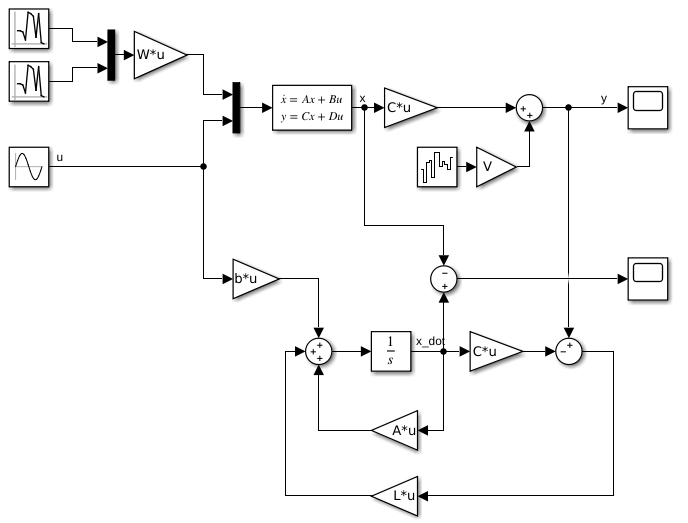
\includegraphics[width=0.6\textwidth]{system}
		\caption{Замкнутая система}
		\label{fig:system}
	\end{figure}
	
	\begin{figure}[H]
		\centering
		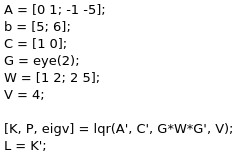
\includegraphics{properties}
		\caption{Параметры системы}
		\label{fig:properties}
	\end{figure}

	Произведем моделирование системы при начальных условиях $x(0)=[1,0]^T$ для $u = sint$. Полученные графики представлены на рисунке \ref{fig:e-2}.
	
	\begin{figure}[H]
		\centering
		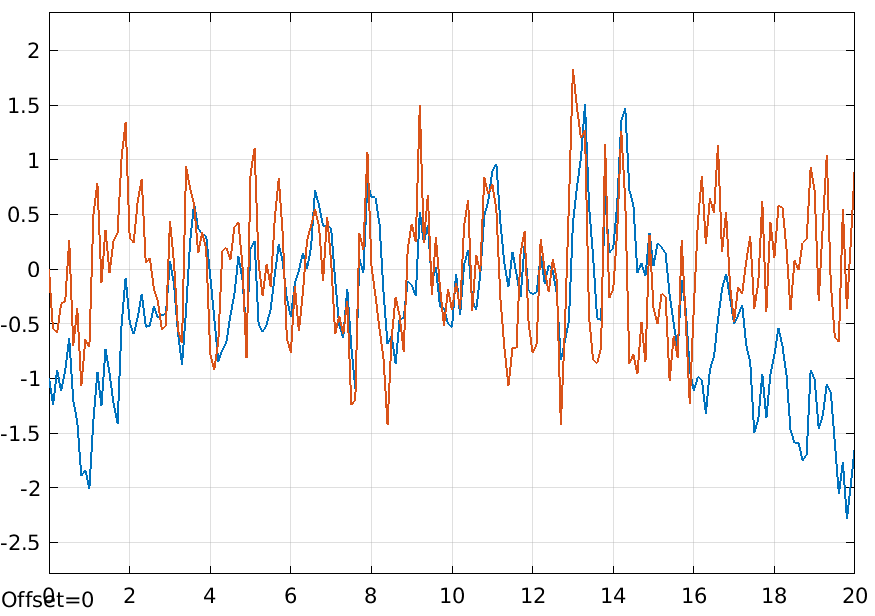
\includegraphics[width=0.6\textwidth]{e-2}
		\caption{Вектор $e_\text{н}$ при $x(0)=[1,0]^T$}
		\label{fig:e-2}
	\end{figure}
	
	Теперь незначительно отклоним расчетное значение $L$ в положительную сторону $L+1$. Полученные графики представлены на рисунке \ref{fig:e-3-plus}.
	
	\begin{figure}[H]
		\centering
		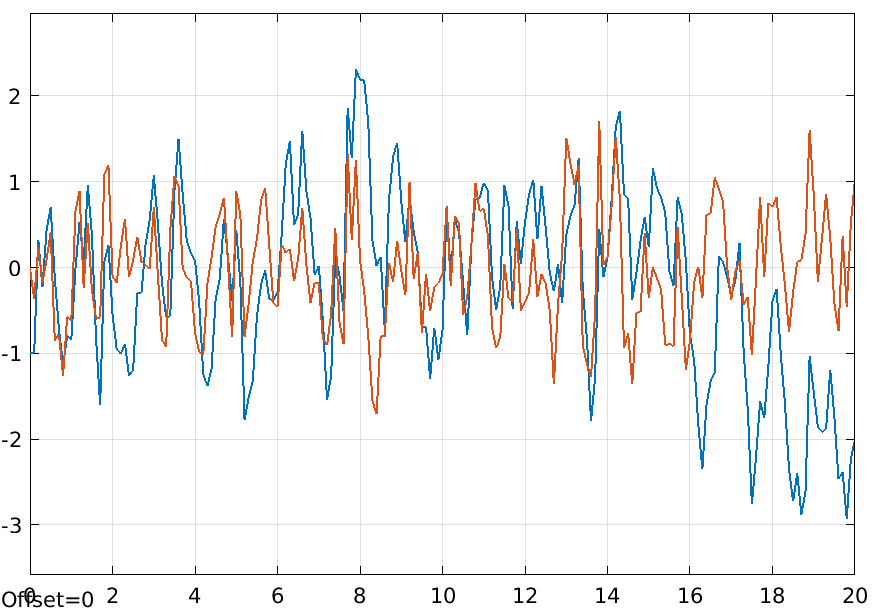
\includegraphics[width=0.6\textwidth]{e-3-plus}
		\caption{Вектор $e_\text{н}$ при $L+1$}
		\label{fig:e-3-plus}
	\end{figure}
	
	При отрицательном отклонении $L-1$ наблюдатель расходится, поэтому промоделируем систему при $L-0,5$. Полученные графики представлены на рисунке \ref{fig:e-3-minus}.

	\begin{figure}[H]
		\centering
		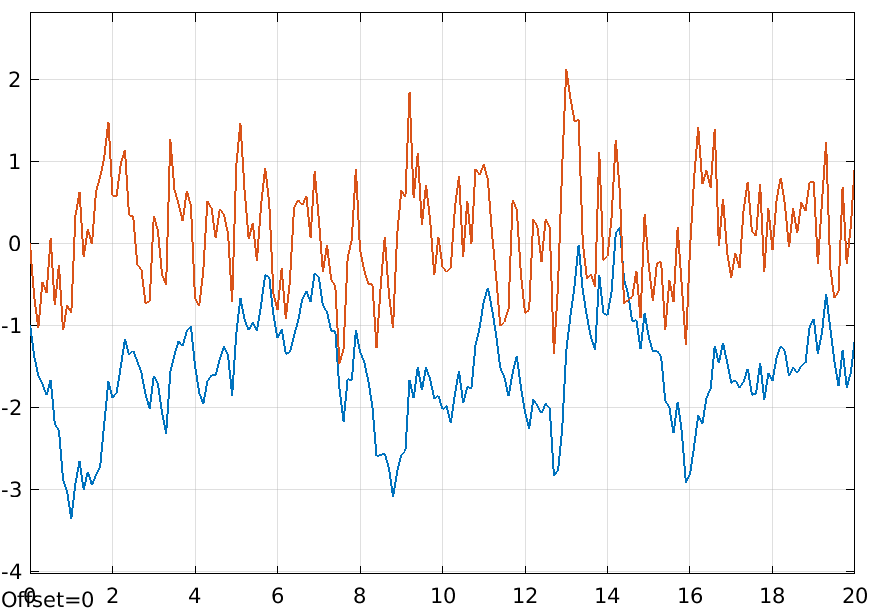
\includegraphics[width=0.6\textwidth]{e-3-minus}
		\caption{Вектор $e_\text{н}$ при $L-0,5$}
		\label{fig:e-3-minus}
	\end{figure}
	
	Проведем моделирование для двух разных матриц $W = kW$. Полученные графики при $k=0,5$, $k=2$ представлены на рисунках \ref{fig:e-4-W05},\ref{fig:e-4-W2}.
	
	\begin{figure}[H]
		\centering
		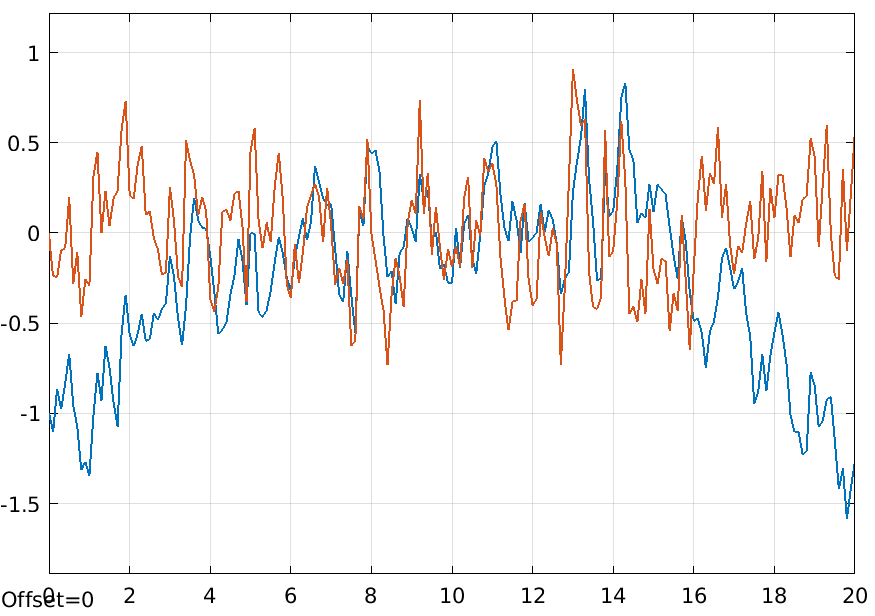
\includegraphics[width=0.6\textwidth]{e-4-W05}
		\caption{Вектор $e_\text{н}$ при $k=0,5$}
		\label{fig:e-4-W05}
	\end{figure}
	
	\begin{figure}[H]
		\centering
		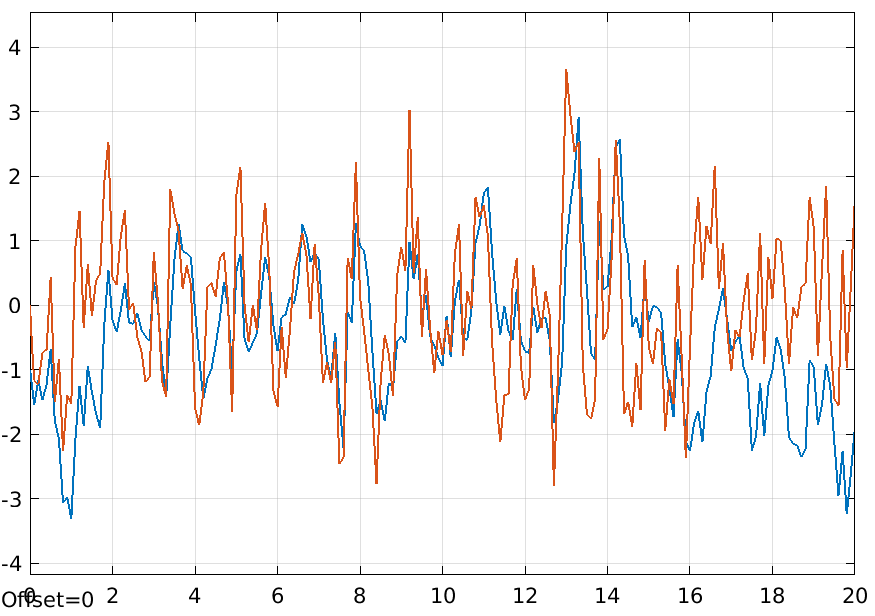
\includegraphics[width=0.6\textwidth]{e-4-W2}
		\caption{Вектор $e_\text{н}$ при $k=2$}
		\label{fig:e-4-W2}
	\end{figure}
	
	Также проведем моделирование для двух разных значений параметра $V$. Полученные графики при $V=2$, $V=6$ представлены на рисунках \ref{fig:e-5-V2}, \ref{fig:e-5-V6}.
	
	\begin{figure}[H]
		\centering
		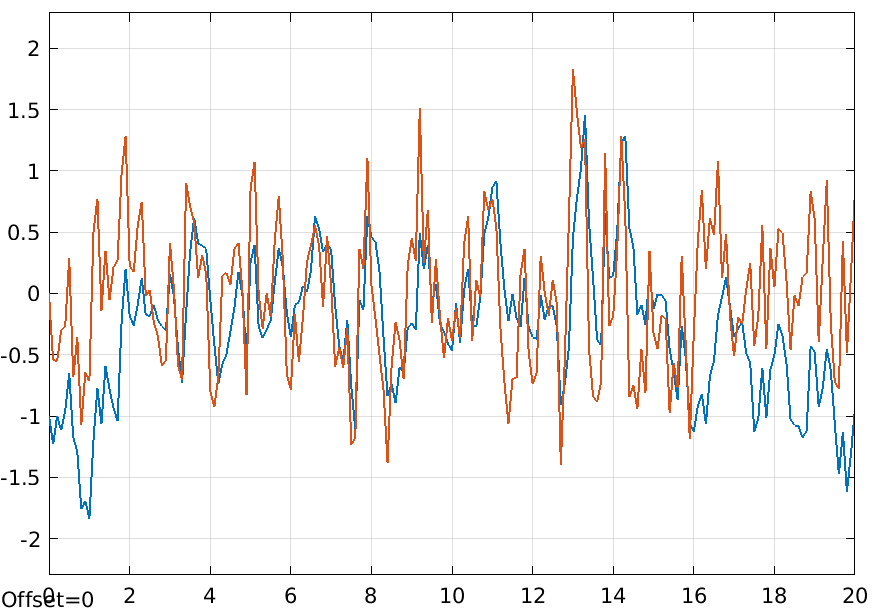
\includegraphics[width=0.6\textwidth]{e-5-V2}
		\caption{Вектор $e_\text{н}$ при $V=2$}
		\label{fig:e-5-V2}
	\end{figure}
	
	\begin{figure}[H]
		\centering
		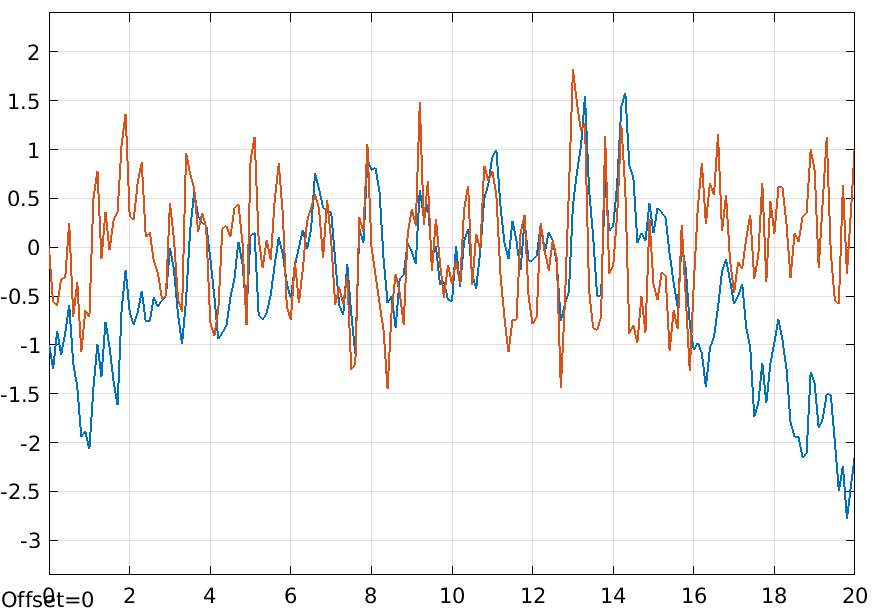
\includegraphics[width=0.6\textwidth]{e-5-V6}
		\caption{Вектор $e_\text{н}$ при $V=6$}
		\label{fig:e-5-V6}
	\end{figure}
	
	\newpage
	
	\section*{Вывод}
	
	При отклонении параметров наблюдателя увеличивается максимальная ошибка $\Delta$, что означает правильность построения оптимального наблюдателя.
	
	
	Значения критерия оптимальности $J$ не были представлены, потому что в данной работе он выражен в виде математического ожидания, которое при моделировании невозможно вычислить в реальном времени.
\end{document}